\chapter{Conclusiones}

\section{Grado de consecución de los objetivos}

Los objetivos planteados en el Apartado\ref{sec:Objetivo} se han alcanzado totalmente. Tras varios meses de trabajo y dificultades, se ha logrado crear un servidor plenamente operativo utilizando lenguaje Erlang OTP que permite lanzar la lectura de ciertos sensores y visualizar los datos obtenidos por los mismos. Este servidor dispone de un manual de uso para que el usuario entienda sin dificultad el funcionamiento de la API REST creada y a su vez está pensado para que un administrador pueda crear más funcionalidad añadiendo o quitando sensores de manera sencilla.

Se ha conseguido un servidor usando Cowboy, que funciona de manera eficiente y con un rendimiento que sobrepasa las necesidades requeridas por parte del sistema y todo ello implementado sobre una Raspberry-Pi 3, por lo que se trata de un sistema portable y fácilmente implementable.

\section{Dificultades encontradas}

En el transcurso del proyecto han aparecido ciertos obstáculos que se han tenido que solventar, se han dividido en dos: problemas con los sensores y problemas con Erlang OTP.

En primer lugar, al comienzo del proyecto, tras la configuración de la placa R-Pi, surgieron problemas con la conexión del sensor MPU6050, el principal problema fue que la placa R-Pi no detectaba de manera correcta el sensor, se probaron sus dos tipos posibles de conexiones (SPI e I2C) y tras varios días de intentos fallidos se decidió descartar este sensor y se sustituyó por el sensor de ultrasonido HC-SR04. Este tipo de conexiones son sencillas y su uso es habitual por lo que no se contaba con tener este tipo de problemas.

Por otro lado, surgieron problemas de incompatibilidad entre los diferentes tipos de servidores posibles a implementar utilizando Erlang OTP sobre la placa R-Pi, esto ha ocurrido debido a que están pensados para ser ejecutados sobre Linux y algunas de las librerías de Raspbian están algo anticuadas o no son compatibles con las de Erlang, se probaron varias opciones de servidores y librerías y finalmente se decidió utilizar Cowboy por su fácil instalación y uso.

Finalmente, el lanzamiento de los sensores desde el servidor no fue fácil debido a los protocolos de seguridad que utiliza Cowboy sobre Erlang, la idea inicial era directamente lanzar el comando usando funciones Erlang como <<cmd>> pero los programas no eran lanzados correctamente ni los datos almacenados en el lugar esperado, es por ello que al final se ha usado Erlang ports para crear una conexión a través de un puerto desde el servidor a la placa R-Pi y de esta manera ejecutar código almacenado en la misma. Para almacenar los archivos en el lugar deseado simplemente se guardan en el servidor (el propio programa lo almacena ahí) y este lo puede leer de su propio directorio.


\section{Desviaciones sobre la planificación}

\subsection{Desviaciones temporales}
El trabajo se inició el día 20 de febrero de 2023 y su fecha final estimada era el 4 de julio. Finalmente con las dificultades encontradas y por otro lado los avances con respecto al tiempo estimado realizados en alguna de las actividades se ha finalizado el proyecto con 6 días de retraso. Este retraso no ha sido considerado un grave problema ya que se ha llegado a la fecha límite de entrega del trabajo y se han cumplido las tareas propuestas.
En la Figura~\ref{fig:gantReal} se muestra la diferencia entre el diagrama Gantt previsto y el Gantt real, con rojo marcado donde ha habido retrasos y verde donde se han realizado las tareas en menor tiempo del previsto.

\begin{figure}[h]
\centering
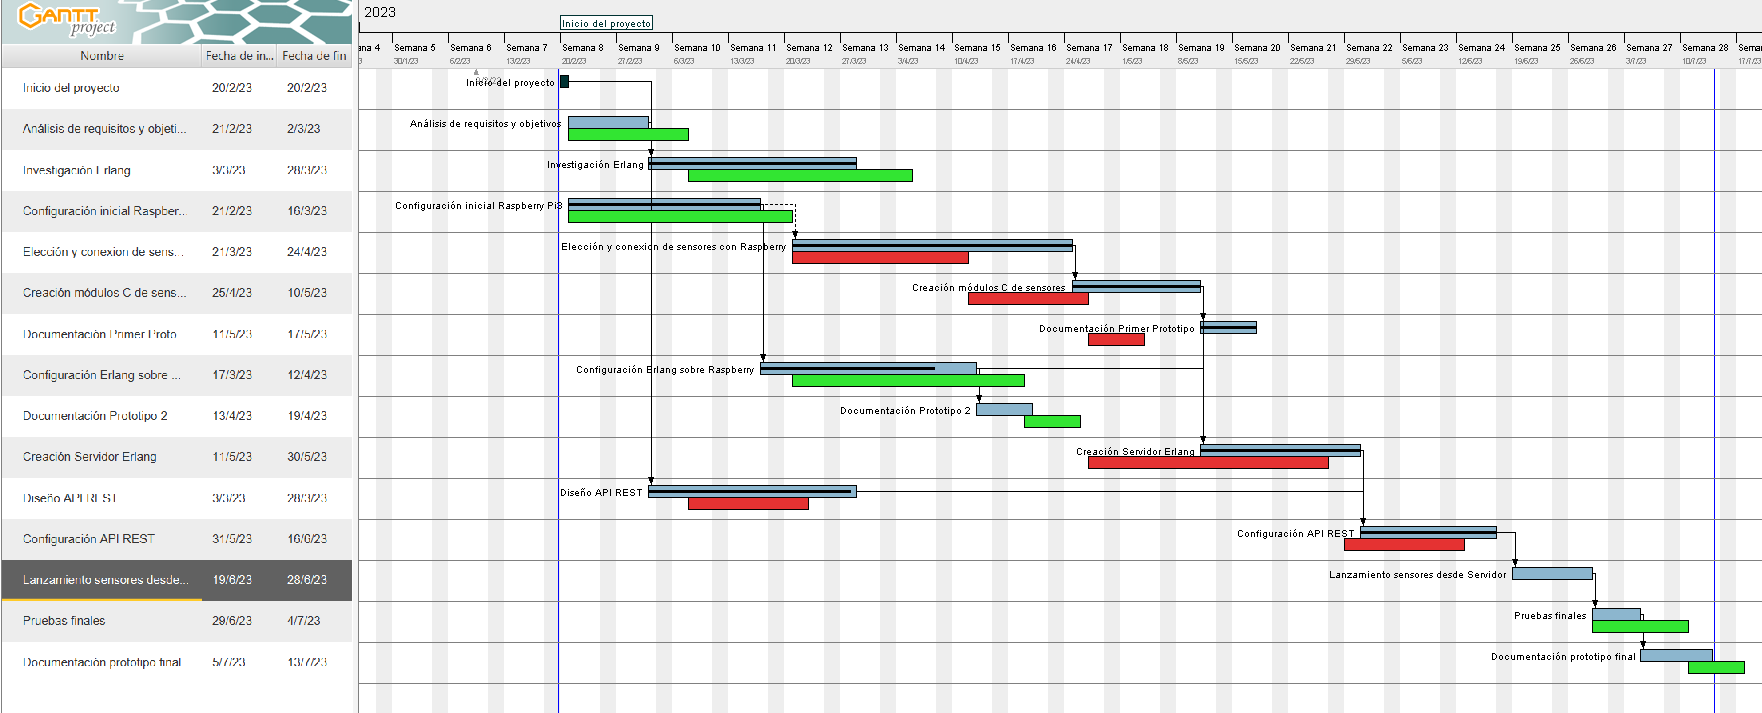
\includegraphics[scale=0.48]{images/gantProyectReal.png}
\caption[Diagrama de Gantt final]{Diagrama de Gantt real con avances y retraso (azul) frente al diagrama Gantt de la planificación inicial (rojo).}%
\label{fig:gantReal}
\end{figure}

\subsection{Desviaciones en presupuesto}

Una diferencia que si que ha sido notable con respecto a la planificación ha sido el número de horas necesarias para la realización del proyecto, debido a que el desarrollador disponía de pocos conocimientos sobre la materia (riesgo valorado en la Sección~\ref{sec:riesgos}) y los problemas comentados en el apartado anterior, el número de horas de trabajo ha aumentado en 120, lo que conlleva a un aumento del presupuesto total en concepto de recursos humanos. Este aumento ha sido de 2280\texteuro{} , por lo que el presupuesto ha pasado de los 6000\texteuro{}  estimados en el Apartado~\ref{sec:recHumanos} a 8280\texteuro{} .

Por último, el gasto en hardware final ha sido el que se observa en la Tabla~\ref{tab:hardwareFinal}, en ella aparecen las tiendas en las que se han adquirido los componentes y su precio específico, en comparación con lo estimado en la Sección~\ref{sec:recHardware} se ha reducido el coste en 41,71\texteuro{}.

\begin{table}[h!]
\begin{center}
\sffamily
\begin{tabular}{|l|c|c|r|}
\hline
\rowcolor{gray!20}
\textbf{Componente} & \textbf{Tienda} & \textbf{Cantidad}  & \textbf{Precio}  \\
\hline
Kit Raspberry-Pi 3 & Compass DHM projects & 1 & 68,93\officialeuro  \\
\hline
Sensor HMC5983 & Sensorae.com & 1 &  6,69\officialeuro \\
\hline
Sensor MPU6050 & Amazon.com & 1 &  3,49\officialeuro \\
\hline
Sensor HC-SR04 & PcComponentes.es & 1 &  2,68\officialeuro \\
\hline
Jumper Wire Cables & az-delivery.de & 3x40 pcs & 6,99\officialeuro \\
\hline
Resistencias 2.2K\(\Omega\) & Aliexpress.com & 10 pcs & 1,75\officialeuro \\
\hline
Resistencias 1K\(\Omega\) & Aliexpress.com & 10 pcs & 1,75\officialeuro \\
\hline
\rowcolor{gray!20}
\textbf{Total} & & & \textbf{85,29\officialeuro} \\
\hline
\end{tabular}
\caption[Costes definitivos componentes hardware]{Costes definitivos de Hardware utilizado para la realización del proyecto}%
\label{tab:hardwareFinal}
\end{center}
\end{table}

Tras el análisis de los costes reales al finalizar proyecto, se han obtenido diferencias en las horas de trabajo y en los costes hardware, por tanto, esto ha resultado un gasto final de 9360,29\texteuro{} en comparación con los 7122\texteuro{} estimados.

\section{Conocimientos aplicados y aprendizajes obtenidos}

A lo largo del desarrollo de este Trabajo de Fin de Grado se han puesto en práctica gran cantidad de conocimientos aprendidos en diferentes asignaturas, a continuación de enumera cada una de ellas junto con su aplicación en este proyecto:

\begin{itemize}
    \item \textbf{Interacción Persona Computadora}: Se ha utilizado para la gestión de sistemas que interaccionan con usuarios como es el caso del servidor, también para el uso de patrones y diseños fáciles de usar.
    \item \textbf{Sistemas Empotrados y Sistemas Digitales}: Conocimientos aplicados en todo aquello relacionado con la electrónica y el hardware.
    \item \textbf{Fundamentos de Programación}: Conocimientos básicos de programación, en este proyecto se ha utilizado lenguaje C, Python y Erlang OTP.
    \item \textbf{Evaluación de Sistemas Informáticos}: Utilizado para la creación de planes de prueba sobre el servidor para poner a prueba su rendimiento y funcionalidad.
    \item \textbf{Servicios y Sistemas Web junto con Diseño, Administración y Seguridad de Redes}: Para la creación y configuración del Servidor Web así como su interfaz y servicio API REST.
    \item \textbf{Diseño, Integración y Adaptación de Software y Fundamentos de Ingeniería de Software}: Para la planificación y análisis del proyecto mediante la creación de diagramas.    
\end{itemize}

A continuación, se detallan las competencias adquiridas o reforzadas a lo largo del proyecto:

\begin{itemize}
    \item Se ha aprendido a desarrollar un proyecto de este calibre, desde la planificación inicial hasta el análisis de requisitos, los planes de prueba, el análisis de riesgos y la documentación.
    \item Se ha aprendido lenguaje funcional Erlang OTP del que los conocimientos eran nulos, desde su instalación en una placa Raspberry-Pi hasta la creación de un servidor utilizando Cowboy.
    \item Se ha aprendido el funcionamiento de la placa R-Pi y de sus conexiones a hardware externo mediante los pines GPIO.
    \item Se han aumentado los conocimientos de programación en C y Python, especialmente en el uso de librerías para hardware externo como WiringPi.
    \item Se ha aprendido sobre protocolos de comunicación entre dispositivos, sus puertos y sus conexiones.
    \item Se ha descubierto el uso de SysML para la creación de diferentes diagramas que permiten el análisis y descripción de proyectos de estas características.
\end{itemize}

\section{Trabajo futuro}

El trabajo descrito en este documento está pensado para permitir a un administrador diversas ampliaciones futuras. El objetivo principal de cara al trabajo futuro era ofrecer un diseño del servidor sencillo y un manual de uso e instalación de las herramientas que permitiera a un administrador añadir o eliminar funcionalidad del sistema, sobretodo en el ámbito de los sensores. Las principales lineas a seguir son:

\begin{itemize}
    \item Crear una interfaz web más visual que permita al usuario moverse de manera más cómoda.
    \item Ampliar la cantidad de sensores, cada uno con una tarea diferente para poder monitorizar un sistema y que estos puedan ejecutarse de manera simultánea.
    \item Acceso a la información captada por los sensores en tiempo real, esto permitiría observar los datos de los sensores en directo para así tomar las medidas necesarias. Actualmente estos datos se leen y se almacenan en archivos que, tras la finalización de la lectura, son visualizables.
    \item Crear un prototipo portable compacto. Actualmente el prototipo físico se ha creado únicamente para pruebas con los sensores y no se ha diseñado un prototipo que sea resistente a golpes, humedad, transportable ni con conexiones sencillas como usb o tipo C para la conexión de los sensores.
    
\end{itemize}

\section{Conclusiones finales}

Tras la realización de este proyecto utilizando Erlang OTP como lenguaje principal, pueden obtenerse algunas conclusiones sobre este tipo de lenguaje para proyectos de estas características.

 Aunque Erlang OTP se desarrolló originalmente para aplicaciones de telecomunicaciones, también se ha utilizado con éxito en una amplia gama de otros dominios, incluyendo, como es el caso, servidores y sistemas embebidos como la Raspberry Pi. Se han descubierto grandes ventajas de este lenguaje a lo largo del proyecto, entre ellas:

 \begin{itemize}
     \item \textbf{La concurrencia}: Tras las pruebas realizadas con gran cantidad de usuarios se ha observado que un servidor sencillo como Cowboy implementado con Erlang, responde muy bien a grandes cantidades de hilos accediendo a la vez. Teniendo en cuenta que está siendo ejecutado sobre un sistema con limitaciones como lo es la Raspberry-Pi, denota un gran punto positivo para Erlang que el rendimiento sea tan bueno.
     \item \textbf{La tolerancia a fallos}: Una gran ventaja de la utilización de Erlang es que sus módulos implementan de manera interna una alta tolerancia a fallos. A lo largo de este proyecto, esta resolución de fallos se ha podido observar en diversas ocasiones y ha resultado muy útil en el marco de la creación de un Servidor Web.  Esto es especialmente importante en entornos donde la fiabilidad es crítica, como la recolección de datos de sensores. Si un sensor falla o se produce un error en el servidor, Erlang OTP permite manejar y recuperarse de manera controlada, evitando que el sistema se caiga por completo.
     \item \textbf{La mensajería y comunicación}:  Erlang OTP proporciona un modelo de programación basado en el intercambio de mensajes ligeros entre procesos. Esto es especialmente útil cuando necesitas comunicarte entre los diferentes componentes de tu sistema de recolección de datos, como en el caso de los sensores. Puede utilizarse este modelo de mensajes para coordinar la lectura de sensores, procesar los datos recibidos y enviar las respuestas a otros componentes del sistema.
    \item \textbf{La escalabilidad}: Los servidores basados en Erlang y especialmente Cowboy, están diseñados para escalar verticalmente y horizontalmente de manera efectiva. Esto significa se puede agregar más capacidad de procesamiento y recursos a medida que crece la cantidad de sensores o la carga de trabajo. La Raspberry Pi tiene recursos limitados en comparación con servidores más potentes, pero Erlang/OTP te permite aprovechar al máximo los recursos disponibles y escalar el sistema de manera eficiente.
 \end{itemize}

Por otro lado, también se han encontrado desventajas en el uso de Erlang, a continuación se describen las más importantes:

\begin{itemize}
    \item \textbf{Gran curva de aprendizaje}: Erlang/OTP sigue un paradigma de programación funcional, que puede diferir significativamente de los enfoques más comunes de programación imperativa o orientada a objetos vistos a lo largo de la carrera, lo que conlleva a que puede haber una curva de aprendizaje pronunciada para los desarrolladores que no están familiarizados con el lenguaje y las convenciones de Erlang/OTP, como ha sido el caso. Esto puede requerir tiempo y esfuerzo adicional para comprender y aprovechar al máximo la plataforma y un cambio de mentalidad y ajuste en la forma de abordar el diseño y la implementación del sistema.
    \item \textbf{Baja disponibilidad de bibliotecas y herramientas}: Aunque Erlang/OTP cuenta con una sólida biblioteca estándar, puede haber limitaciones en cuanto a la disponibilidad de bibliotecas y herramientas de terceros en comparación con otros lenguajes y plataformas más populares. Esto puede dificultar la integración con determinados componentes o servicios externos que podrían ser necesarios en el proyecto. Para ciertos componentes, sobretodo hardware externo utilizado en Raspberry-Pi, existe mucha información con el uso de Python, pero Erlang no es tan utilizado y esto lleva a que las búsquedas sean mucho más tediosas.
    
    \item \textbf{Menor comunidad y soporte}: Aunque Erlang/OTP cuenta con una comunidad activa de desarrolladores, su tamaño y alcance son más limitados en comparación con otros lenguajes y plataformas más populares, esto se observa de manera muy habitual cuando vamos a realizar una búsqueda sobre cuestiones específicas del sistema, en otros lenguajes existen muchos casos de fallos comunes o foros de preguntas y respuestas pero en el caso de Erlang es mucho más limitado y muchas veces anticuado. Esto podría resultar en una disponibilidad reducida de recursos de aprendizaje, documentación y soporte en línea, lo que podría dificultar la resolución de problemas o la obtención de ayuda en momentos críticos.
    
\end{itemize}

\appendix

\chapter{Contenido Digital}
\section{Contenido del repositorio}

Todo el código de este proyecto ha sido almacenado en la cuenta personal del alumno en Github de manera pública. En este repositorio se puede encontrar:\\

\dirtree{%
.1 HCSR04. 
.2 distance\_sensor.py: Código Python del sensor HC-SR04.
.2 ultrasonido.c: Código C del sensor HC-SR04. 
.1 HMC5983.
.2 i2c.py: Código Python del sensor HMC5983.
.2 cabeceoArchivo.c: Código C del sensor HMC5983.
.1 cowboyServer.
.2 sensorData: Almacena los datos obtenidos por los sensores.
.3 angulosCabeceo.txt: Datos del sensor HMC5983.
.3 distancias.txt: Datos del sensor HC-SR04.
.2 text: Almacena los JSON descriptores de sensores.
.3 inicio.json.
.3 magnetometro.json.
.3 sensores.json.
.3 ultrasonido.json.
.2 data\_handler.erl.
.2 hello\_erlang\_app.erl.
.2 hello\_erlang\_sup.erl.
.2 hello\_handler.erl.
.2 launch\_handler.erl.
.2 not\_found\_hanlder.erl.
.2 update\_handler.erl.
.1 TFG\_Martin\_Tornero.zip: Documentación del proyecto.
.1 README.md: manual de uso e instalación.
}

\section{Manual de instalación}

En las carpetas de los sensores encontramos dos archivos: Programa en C y programa en Python. El utilizado por el servidor es el programa en C. Para ejecutar los programas en C estos deben compilarse utilizando sus librerías. 

\begin{itemize}
    \item En el caso del sensor de ultrasonido HC-SR04 debe compilarse la librería WiringPi.h de la siguiente manera:
    \begin{lstlisting}[style=terminal]
    gcc -o ultrasonido ultrasonido.c -lwiringPi
    \end{lstlisting}
    
    \item En el caso del sensor magnetómetro HMC5983 debe compilarse la librería pigpio.h mediante el comando: 
     \begin{lstlisting}[style=terminal]
    gcc -o cabeceoArchivo cabeceoArchivo.c -lpigpio -lm
    \end{lstlisting}
    
\end{itemize}

Para lanzar el servidor debe disponerse de Erlang instalado y Cowboy configurado correctamente, para ello se recomienda seguir los pasos de la Sección~\ref{sec:ConfigCowboy}. Una vez completada la configuración inicial se pueden descargar los archivos de este repositorio accediendo a la URL \url{https://github.com/martorn/TFGMartinTorneroVazquez.git} o escaneando el código QR disponible en la Figura~\ref{fig:QR}.

\begin{figure}[h]
\centering

\includegraphics[scale=0.48]{images/qr.png}
\caption{Código QR del repositorio GitHub}%
\label{fig:QR}
\end{figure}
    

Por defecto, el servidor es lanzado en localhost sobre el puerto 8080, en caso de querer modificar esto podemos hacerlo de manera sencilla en hello\_erlang\_app.erl en su sección correspondiente. Por otro lado, es posible que surjan errores a la hora de lanzar los códigos de los sensores, es importante que se hayan compilado con anterioridad e indicar al servidor el lugar de almacenamiento del ejecutable del archivo y la localización de los archivos creados que almacenan los datos de los sensores. Estas modificaciones deben realizarse sobre el archivo launch\_handler.erl en sus funciones correspondientes.

Finalmente, si los pasos se han realizado correctamente, podemos lanzar el servidor ejecutando <<make run>> y acceder al mismo usando curl o a través de un navegador.

Los datos del repositorio han sido actualizados en Julio de 2023.